\documentclass[10pt,a4paper]{article}
\usepackage[margin=1in]{geometry}
\usepackage{xeCJK}
%\usepackage{indentfirst}
\usepackage{enumitem}
\usepackage{setspace}
\usepackage{float}
\usepackage{calc}
\usepackage{amsmath}
\setCJKmainfont{AR PL UMing TW}

\usepackage{fancyhdr}
\pagestyle{fancy}
\lhead{WNFA Lab 3 Report}
\chead{}
\rhead{Group 5}
\lfoot{}
\cfoot{}
\rfoot{\thepage}
\renewcommand{\headrulewidth}{0.4pt}
\renewcommand{\footrulewidth}{0.4pt}

\setlength{\parindent}{0pt}
\setlength{\parskip}{.4em}
\linespread{1.15}

\begin{document}
\thispagestyle{fancy}

\begin{center}
    \LARGE WNFA Lab 3 Report
\end{center}
\begin{center}\begin{tabular}{lccr}
    Group 5: & B02902125吳哲宇 & B01902010李紹詮 & B01902048王欣維 \\
    & B01902085邱劭同 & B01902138蔡存哲
\end{tabular}\end{center}

\section*{工作原理}
USRP收發訊號:使用助教提供的\texttt{signal\_generator.m}產生訊號後,透過UHD API送出/接收訊號。發送端透過\texttt{usrp->get\_device->send()}不斷送出同一訊號,每份訊號中間有間隔。接收端則以\texttt{usrp->get\_device->recv()}接收一定時間內的訊號,交由MATLAB code做後續處理。

\begin{figure}[h]
    \centering
    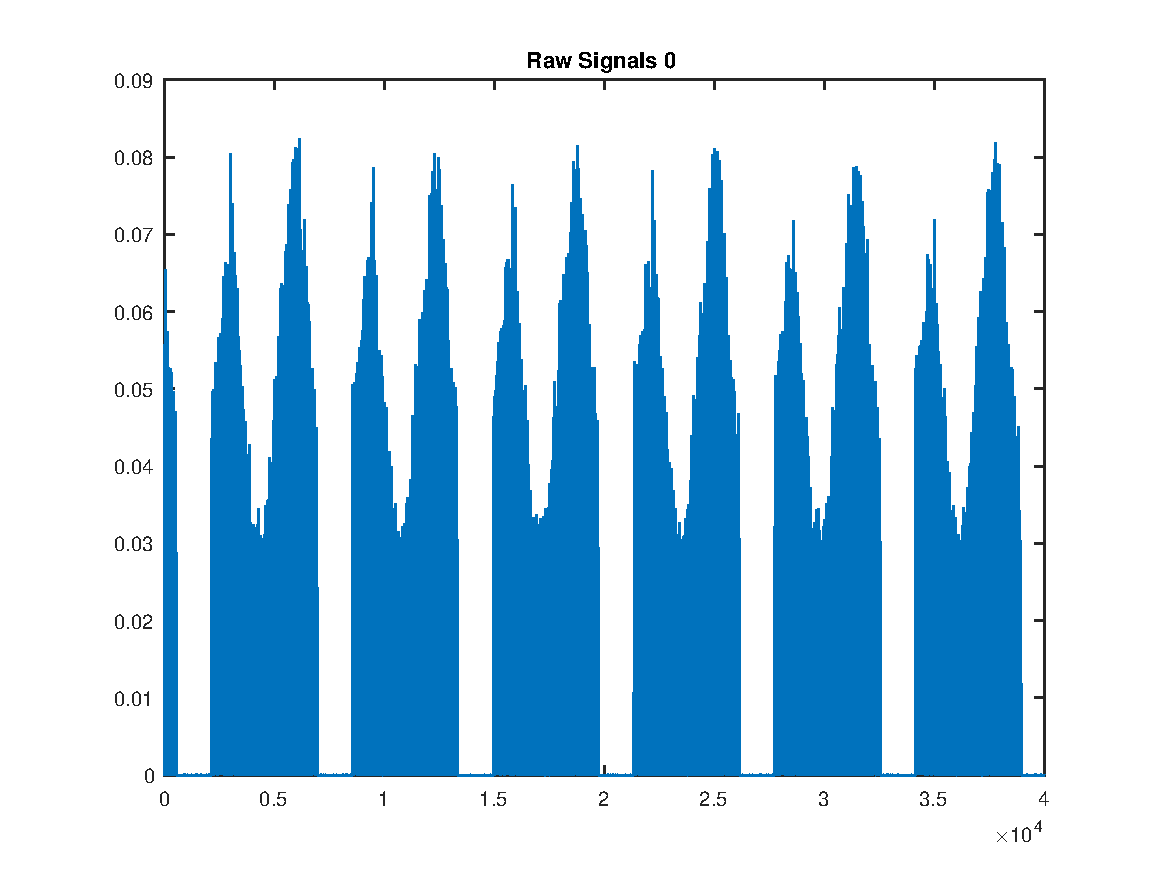
\includegraphics[trim=30 10 30 10,clip,width=0.6\linewidth]
    {figures/raw_signal}
    \caption{透過USRP接收到的raw signal}
\end{figure}

MATLAB封包解析:對於接收到的訊號依序做以下計算:
\begin{enumerate}
    \item packet detection: 計算訊號的cross-correlation以偵測preamble位置。由前往後掃描訊號,對每個preamble長度的window計算correlation。當correlation高於設定的threshold時,開始記錄correlation的最大值以及window位置,直到correlation降到低於threshold時,回傳先前記錄correlation最大的位置作為封包的preamble位置。
    \item CFO correction: 使用助教提供的 function \\
    \hspace*{-\leftmargin}
    \begin{minipage}{\linewidth+\leftmargin}
        \centering
        \begin{minipage}{0.45\linewidth}
            \begin{figure}[H]
                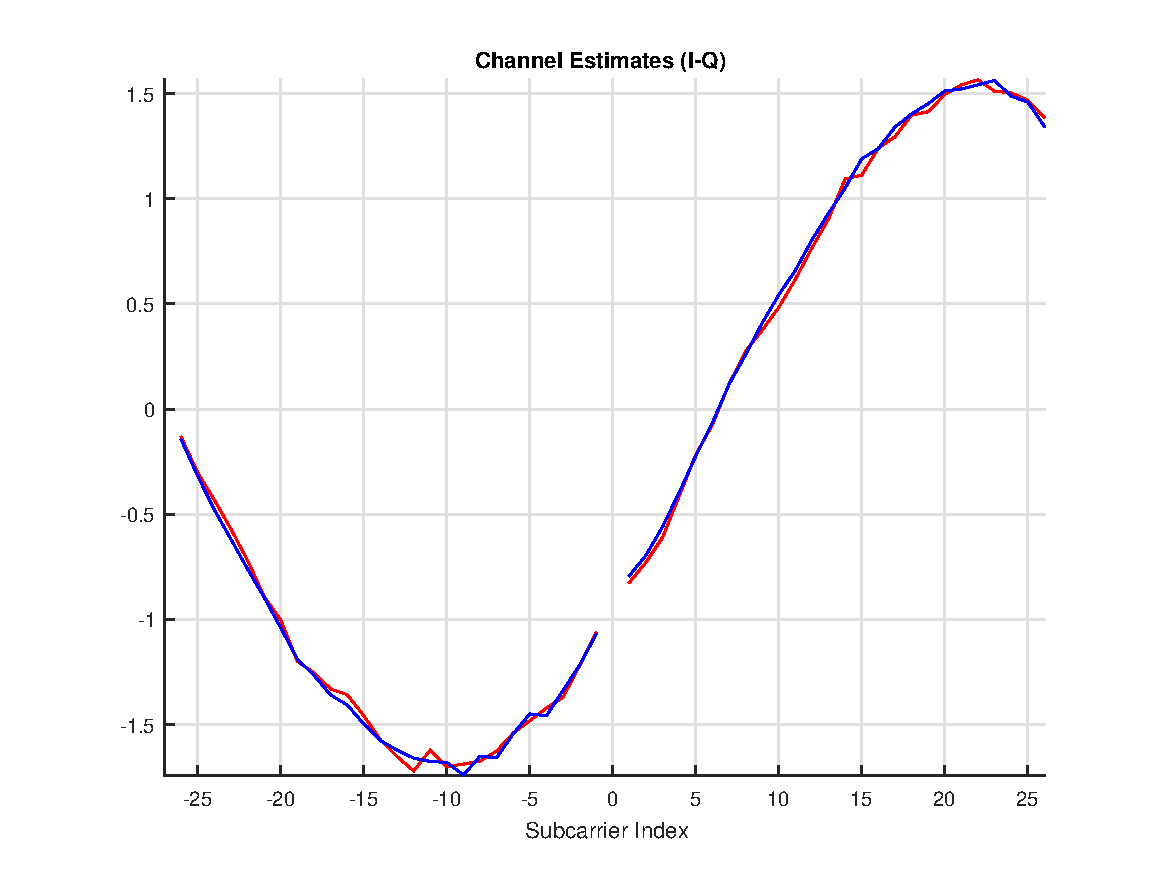
\includegraphics[trim=30 10 30 10,clip,width=\linewidth]
                {figures/channel_1}
                \caption{channel estimates of preamble}
            \end{figure}
        \end{minipage}
        \begin{minipage}{0.45\linewidth}
            \begin{figure}[H]
                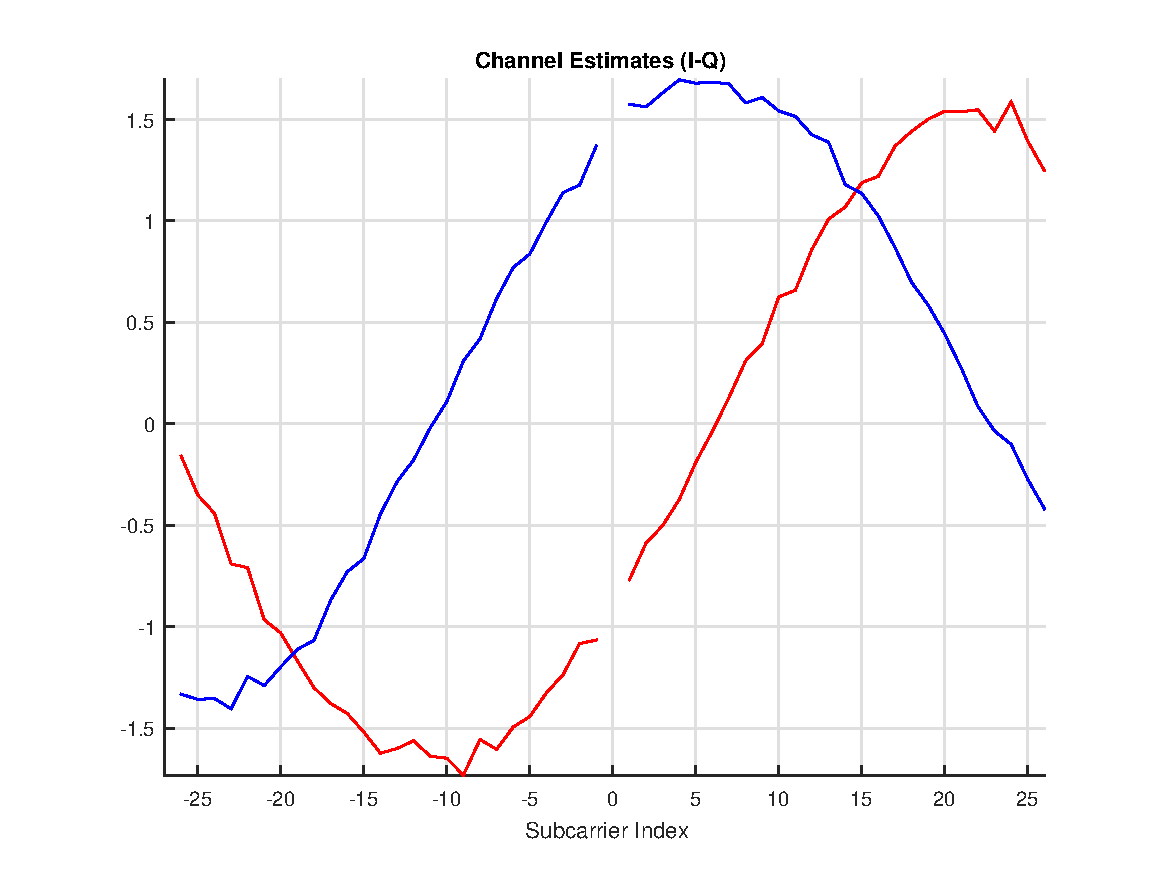
\includegraphics[trim=30 10 30 10,clip,width=\linewidth]
                {figures/channel_2}
                \caption{channel estimates of payload}
            \end{figure}
        \end{minipage}
    \end{minipage}
    \item 移除cyclic prefix
    \item phase tracking: 利用封包內帶的pilot bits,對pilot bits做linear regression (實作中使用MATLAB degree-1 polyfit,等同於 linear regression),得出在不同subcarrier上的偏移後,即可實施SFO correction。
    \item 得到BPSK symbols,decode完成
\end{enumerate}

\begin{minipage}{\linewidth}
    \centering
    \begin{minipage}{0.45\linewidth}
        \begin{figure}[H]
            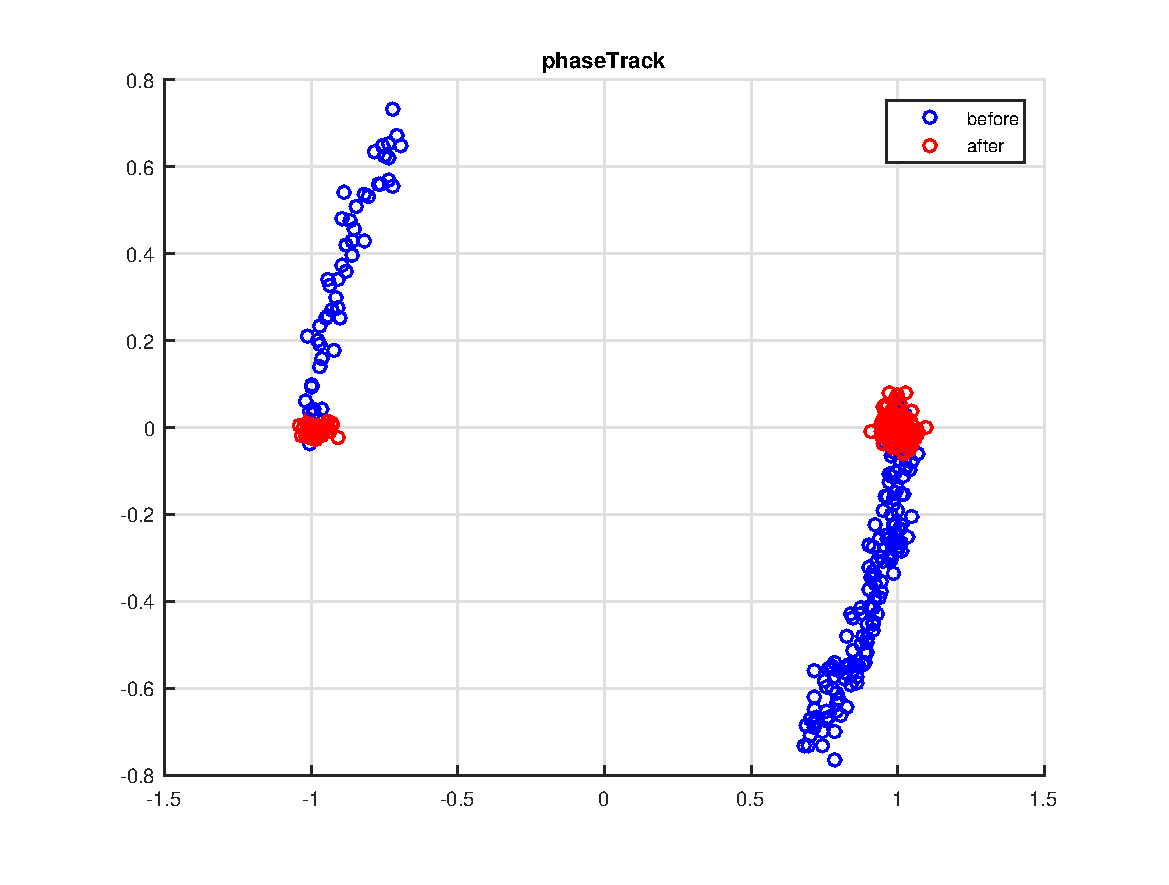
\includegraphics[trim=30 10 30 10,clip,width=\linewidth]
            {figures/phase_track}
            \caption{phase tracking前/後的symbols比較}
        \end{figure}
    \end{minipage}
    \begin{minipage}{0.45\linewidth}
        \begin{figure}[H]
            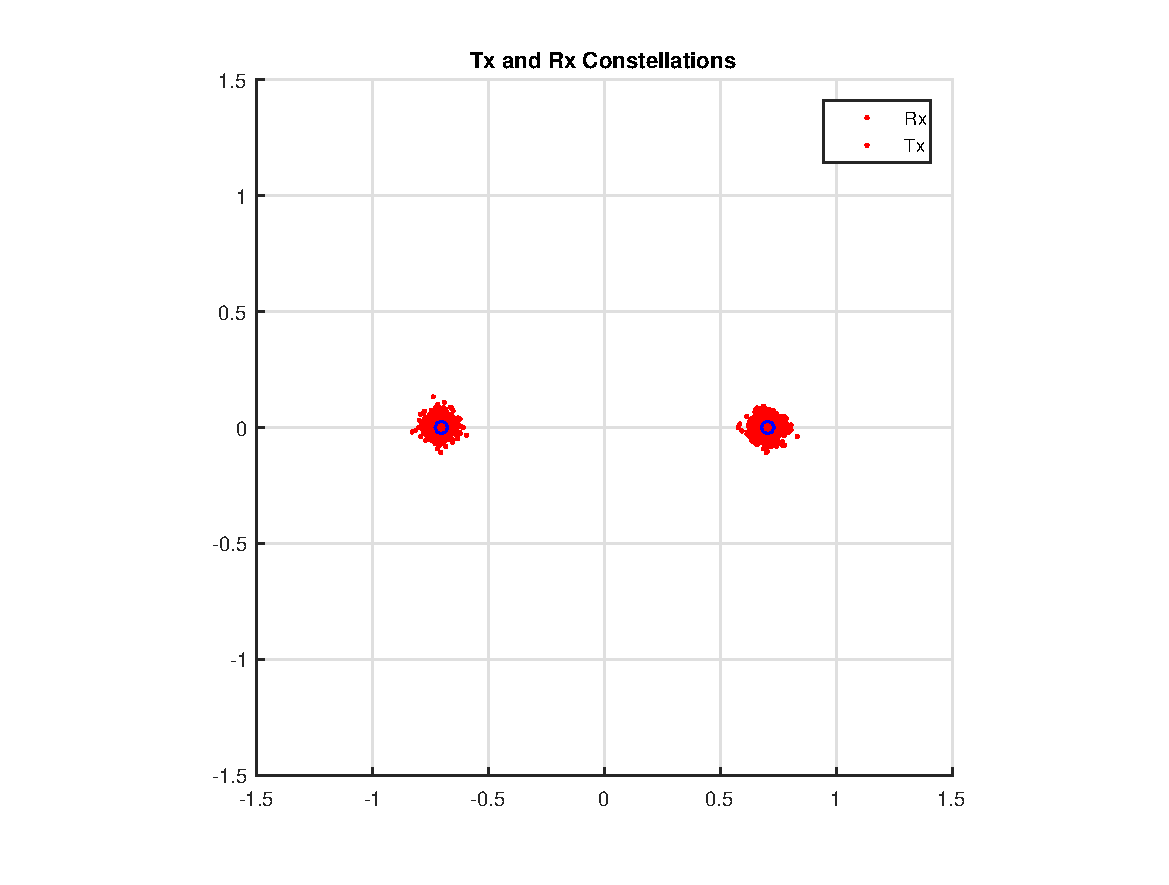
\includegraphics[trim=30 10 30 10,clip,width=\linewidth]
            {figures/constellations}
            \caption{BPSK symbols}
        \end{figure}
    \end{minipage}
\end{minipage}

\vspace{1em}
SNR計算:令SNR為$\gamma$,symbols平均強度為$\rho$,symbols變異數為$\sigma$,則:
\begin{equation}\label{eq:SNR}
\gamma = \frac{(\frac{1}{\rho})^2}{\sigma^2}
\end{equation}
利用\eqref{eq:SNR}計算各subcarrier以及各symbol的SNR。

\begin{minipage}{\linewidth}
    \centering
    \begin{minipage}{0.45\linewidth}
        \begin{figure}[H]
            \includegraphics[trim=30 10 30 10,clip,width=\linewidth]
            {figures/snr_subcarrier}
            \caption{各subcarrier的SNR}
        \end{figure}
    \end{minipage}
    \begin{minipage}{0.45\linewidth}
        \begin{figure}[H]
            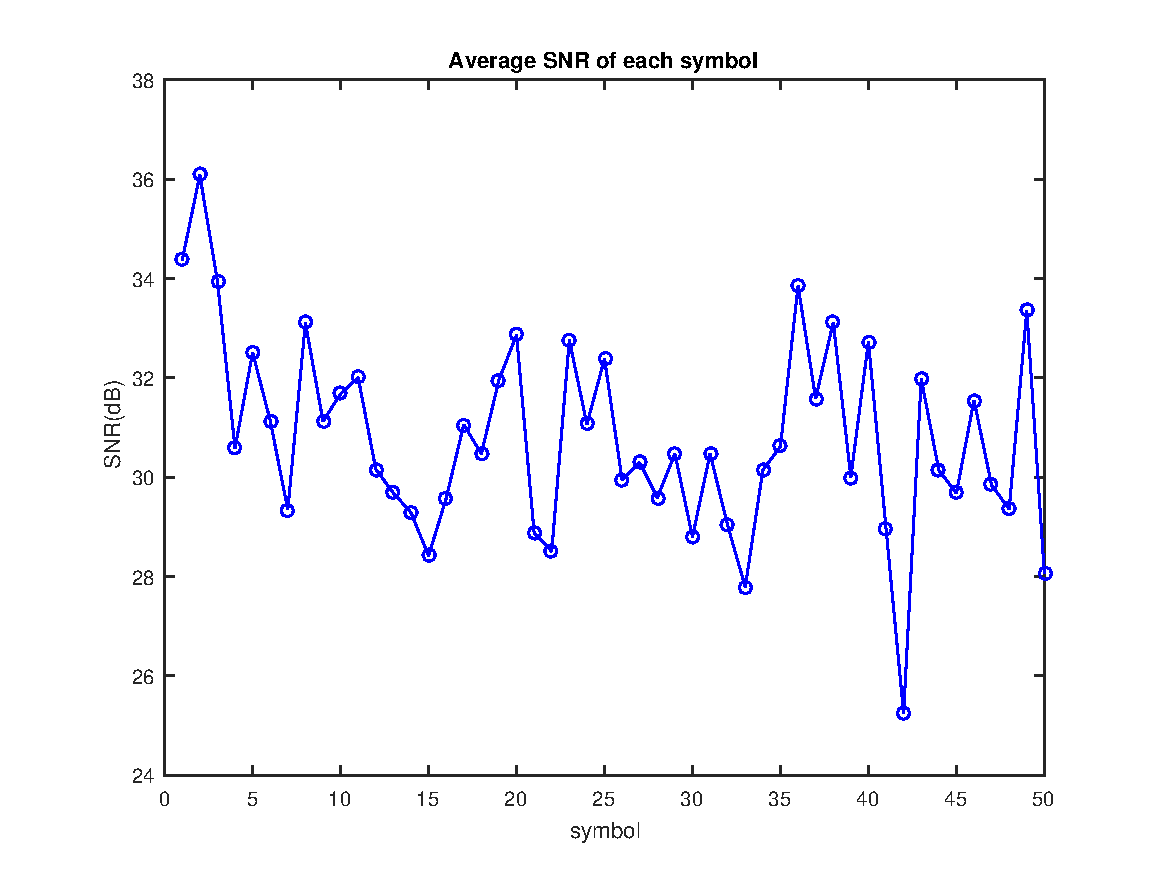
\includegraphics[trim=30 10 30 10,clip,width=\linewidth]
            {figures/snr_symbol}
            \caption{各symbol的SNR}
        \end{figure}
    \end{minipage}
\end{minipage}

\pagebreak

\section*{遇到的問題 \& 解決方法}
\begin{enumerate}
    \item 在接上USRP之前無法測試接收訊號。\\
    Solution: 利用訊號處理library ``IT++''提供的Rayleigh fading process來模擬原始訊號在傳輸過程中的改變。
    \item USRP接收到的訊號在距離僅5公尺左右時就已經弱到無法辨識。\\
    Solution: 提高接收端天線的gain (預設值是30,透過參數\texttt{--g=<gain>}提高到50左右即可)
\end{enumerate}

\section*{工作分配}
\begin{itemize}[leftmargin=!,itemindent=-4em]
    \item 吳哲宇:packet detection實作,phase tracking實作,模擬接收訊號
    \item 李紹詮:透過UHD API操作USRP實作,SNR計算實作,報告統整
    \item 邱劭同:準備final project proposal
\end{itemize}

\end{document}
